\documentclass[a4paper,11pt]{article}
\usepackage{dmasproject}
% if you need additional LaTeX packages, add them here

\title{Simulating the Effect of Social Media on Civil Violence}
% sort your names alphabetically by last name
\author{
  Rafael Tappe Maestro (s3258734)
  \\
  Arseniy Nikonov (s2977419)
  \\
  Panagiotis Ritas (s3152529)
  \\
  Tobias van der Werff (s4314719)
}
%\date{Alpha version, September 2020} % change this accordingly
\date{State of the Art analysis, September 2020}

\begin{document}

\maketitle

\begin{abstract}
The abstract should briefly summarize your project in 150--250 words.
\end{abstract}

\section{Introduction}

Social media adds a new dimension to the dynamics of civil protests. The Arab spring provides a clear example of protests fueled by social media: it has been argued that social media played an instrumental role in the success of the anti-government protests ~\cite{eltantawy2011arab} and that online revolutionary conversations often preceded major events on the ground ~\cite{howard2011opening}. Moreover, a 2011 survey of participants in Egypt’s  Tahrir Square protests indicates that social media use greatly increased the  odds of respondents attending protests on the first day ~\cite{tufekci2012social}.  In this paper we focus on the effect that social media has on the dynamics of civil violence when it is used to fuel both new and existing protests. 

\subsection{State of the art}

We use Epstein’s model of civil violence ~\cite{epstein2002modeling} as a starting point for our model. Epstein’s paper provides an agent based simulation of civil violence. In this simulation, protesters rebel against authority (cops) in an environment resembling a riot. We will be focusing on one out of two models presented in Epstein’s paper, in which agents in authority aim to suppress and imprison the group of protesters, who are actively rebelling.
    
Protesters can either be passive or be actively rebellious. Each protester's grievance level is influenced by two components: illegitimacy, which is the perceived illegitimacy of the government, as well as hardship, which measures each individual agent's economic privation.  Each agent also has a calculated probability of being arrested. This probability depends on the amount of cops and the amount of already active rebellious protesters in his vision. Hence, more cops in his surroundings means a higher arrest probability, and more active protesters in his surroundings means a lower probability of being arrested. Protesters become active depending on how averse they are on taking risks, on their estimated probability of being arrested, and their given grievance levels. Cops will in general arrest and send to jail protesters that are active within their vision. After a randomly given jail time, protesters return back to the simulation.

These simple rules and components of the simulation provide some interesting findings. Specifically, it was observed that protesters become passive when cops are near, but become rebellious again when cops left their vision. Another observation is that in areas where a lot of rebellious protesters, and at the same time a small number of cops are gathered, there occurs an “uprising", in which most protesters become active and rebel. In general, the simple rules in the model produced some complex and emerging behaviors which represent real life’s political upheavals and protests against authority.


\subsection{New idea}

In this research, we aim to extend Epstein's model of civil violence to include the effects of social media. Epstein's model was published in 2002 and did not include a notion of social media or online discourse in general. However, it seems reasonable to assume that a more modern version of Epstein's model would include the effects of online discourse, since the effects of social media on civil violence can be grave. Contrary to Epstein's model where vision is local and information is limited, the ubiquitousness of social media creates new dynamics where information is abundant and vision is expanded. We will investigate the effect that these changes have on Epstein's model. 

\section{Method}

\subsection{Simulation model}

Here you should describe your model.
How similar to the one used in your state of the art reference is it?
Which things did you change, and why?

\begin{figure}[h]
  \centering
  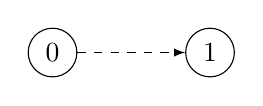
\begin{tikzpicture}[node distance=2cm,>=latex]
    \node (0) [circle,draw] {0};
    \node (1) [circle,draw,right of=0] {1};
    \draw [->,dashed] (0) -- (1);
  \end{tikzpicture}
  \caption{A figure should always have a caption.}\label{fig1:twoDots}
\end{figure}

If you add figures, such as \autoref{fig1:twoDots}, always refer to them at least once.
Please use tikz or vector formats like EPS or PDF.
Avoid pixel formats such as PNG or JPG (because they would become pixelated or blurry).

\subsection{Implementation details}

Here you should describe the implementation of your simulation.
Please explicitly mention any programming languages, tools or libraries you used.

\subsection{Experiment design}

Did you run multiple different versions of your simulation with different parameters?
Then explain the different setups here and why you chose them.

You can also mention here what results you are expecting.

\section{Results}

\subsection{Experiment findings}

Key question 4: What are the results you obtained?

It can be good to use a Table, like \autoref{tab1:results}.
Please ensure that numeric results are right-aligned and have the same number of digits, to allow for easy comparison.

\begin{table}[h]
  \centering
  \begin{tabular}{lrr}
    \toprule
    Setup & run time & success rate \\
    \midrule
    1  & 0.123 & 12\% \\
    2  & 0.456 & 34\% \\
    3a & 0.789 & 56\% \\
    3b & 1.234 & 78\% \\
    \bottomrule
  \end{tabular}
  \caption{Tables should always have a caption.}\label{tab1:results}
\end{table}

You might also want to include plots or graphs.
Similar to figures, please do not use screenshots or pixel-based formats, but vector-based formats.
Alternatively, generate your plots with the \texttt{pgfplots} package as done here in Figure~\ref{fig1:plot}.

\begin{figure}[h]
  \centering
  \begin{tikzpicture}
    % ideally the results.txt file should be automatically generated by your implementation.
    \pgfplotstableread{results.txt}\datatable
    \begin{axis}
      \addplot+[error bars/.cd, y dir=both, y explicit, error bar style={color=black}] table[x=day, y=explosions, y error=explosionsSD] from \datatable;
      \addplot+[error bars/.cd, y dir=both, y explicit, error bar style={color=black}] table[x=day, y=fires, y error=firesSD] from \datatable;
      \legend{explosions, fires};
    \end{axis}
  \end{tikzpicture}
  \caption{Figures should also have a caption.}\label{fig1:plot}
\end{figure}

\subsection{Interpretation of findings}

Summarise your results.
Are the results what you expected?
Which results are surprising?
How do you interpret them?

\section{Conclusion}
\subsection{Discussion}

What do you take away from your project?
What did you learn?

\subsection{Relevance}

Key question 5: What is the relevance of this work?

Which new questions do you have now?
Do you results suggest future research directions?

\subsection{Team Work}

How did you work together as a team?
Who contributed how to this report and to the implementation?
What should you have done differently?

% This will print you references, please do not change it.
\printbibliography

\end{document}
